\documentclass{TIJMUjiaoanLL}
\pagestyle{empty}

\begin{document}

\kecheng{分子生物计算}
\neirong{限制酶图谱和正则表达式 \ / 第9章}
\jiaoshi{伊现富}
\zhicheng{讲师}
\riqi{2019年10月23\&25日10:00-11:40\&13:30-15:10}
\duixiang{生物医学工程与技术学院2017级生信班(本)}
\renshu{28}
\fangshi{理论讲授}
\xueshi{4}
\jiaocai{Perl语言在生物信息学中的应用——基础篇}

\firstHeader
\maketitle
\thispagestyle{empty}

\mudi{
\begin{itemize}
  \item 掌握:正则表达式的基础语法与基本应用;模式匹配中的特殊变量。
  \item 熟悉:逻辑操作符的求值顺序。
  \item 了解:范围操作符的应用。
  \item 自学:操作符的优先级。
\end{itemize}
}

\fenpei{
\begin{itemize}
  \item (5')引言与导入:回顾已经学习的与正则表达式和操作符相关的知识点;介绍将要学习的主要内容。
  \item (80')正则表达式:通过实例介绍正则表达式的应用,详细讲解正则表达式的常量、运算、语法和元字符等基础知识,举例说明正则表达式在生物信息学中的应用。
  \item (80')限制酶切图谱:简单介绍限制酶的背景知识,通过制作酶切图谱的Perl程序详细讲解正则表达式在限制酶切位点分析中的应用。
  \item (10')操作符优先级:简单介绍优先级的概念,总结常见操作符的优先级。
  \item (5')总结与答疑:总结授课内容中的知识点与技能,解答学生疑问。
\end{itemize}
}

\zhongdian{
\begin{itemize}
  \item 重点:正则表达式的基本语法;正则表达式中的元字符;模式匹配中的特殊变量。
  \item 难点:正则表达式的基本语法;逻辑操作符的求值顺序;pos函数的使用。
  \item 解决策略:通过实例演示帮助学生理解、记忆。
\end{itemize}
}

\waiyu{
\vspace*{-10pt}
\begin{multicols}{2}
正则表达式(regular expression)

模式(pattern)

元字符(metacharacter)

优先级(precedence)

限制酶(restriction enzyme)

回文序列(palindrome sequence)

范围操作符(range operator)

逻辑操作符(logical operator)
\end{multicols}
\vspace*{-10pt}
}

\fuzhu{
\begin{itemize}
  \item 多媒体:正则表达式实例;限制酶酶切位点示意图;bionet文件格式。
  \item 板书:逻辑操作符的求值顺序;使用括号明确优先级。
  \item 演示:正则表达式在酶切图谱制作中的应用。
\end{itemize}
}

\sikao{
\vspace*{-10pt}
\begin{multicols}{2}
\begin{itemize}
  \item 总结正则表达式的基本运算。
  \item 总结正则表达式的基本语法。
  \item 举例说明正则表达式中的元字符。
  \item 解析正则表达式实例。
  \item 根据要求编写正则表达式。
  \item 列举常见的逻辑操作符,解释其求值顺序。
  \item 举例说明模式匹配中的特殊变量。
  \item 如何明确复杂表达式中操作的优先级?
\end{itemize}
\end{multicols}
\vspace*{-10pt}
}

\cankao{
\begin{itemize}
  \item Beginning Perl for Bioinformatics, James Tisdall, O'Reilly Media, 2001.
  \item Perl语言入门(第六版),Randal L. Schwartz, brian d foy \& Tom Phoenix著,盛春\ 译,东南大学出版社,2012。
  \item Mastering Perl for Bioinformatics, James Tisdall, O'Reilly Media, 2003.
  \item 维基百科等网络资源。
\end{itemize}
}

\firstTail

\newpage
\otherHeader

\begin{enumerate}
  \item 引言与导入(5分钟)
    \begin{enumerate}
      \item 已经学习
	\begin{itemize}
	  \item Perl语言:模式匹配与字符替换(正则表达式);数字和字符操作符(操作符)
	  \item 生物信息学:处理FASTA格式的文件;在DNA序列中查找基序
	\end{itemize}
      \item 即将学习
	\begin{itemize}
	  \item Perl语言:正则表达式的基本理论;操作符的优先级
	  \item 生物信息学:用正则表达式表征酶切数据;制作酶切图谱
	\end{itemize}
    \end{enumerate}
  \item 正则表达式(80分钟)
    \begin{enumerate}
      \item 简介\textcolor{red}{(日用而不知:文本编辑器中的检索和替换)}
	\\正则表达式使用单个字符串来描述、匹配一系列符合某个句法规则的字符串。
      \item 实例\textcolor{red}{(DNA基序、文本搜索、用户名、电子邮箱、网址等)}
	\begin{itemize}
\parpic[fr]{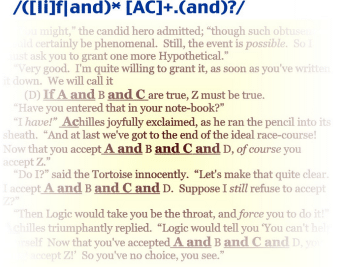
\includegraphics[width=0.38\textwidth]{c9_enzyme_re_text_01.png}}
	  \item \verb|/CT[CGT]ACG/|:完整的正则表示式(基序)
	  \item \verb|//|:正则表达式界定符
	  \item \verb|ACGT|:ACGT四种碱基/四个字符本身
	  \item \verb|[CGT]|:C或者G或者T
	  \item 基序:CTCACG或者CTGACG或者CTTACG
	\end{itemize}
      \item 理论
	\begin{enumerate}
	  \item 基本理论
	    \begin{itemize}
	      \item 简介:常量(字符串的集合) + 算子(集合上的运算)
	      \item 常量:空集,空串,文字字符
	      \item 运算:串接,选择,Kleene星号
	      \item 运算优先级:Kleene星号 $\textgreater$ 串接 $\textgreater$ 选择
	    \end{itemize}
	  \item 基本语法
	    \begin{itemize}
	      \item 简介:一个正则表达式通常被称为一个模式,为用来描述或者匹配一系列符合某个句法规则的字符串。
\parpic[fr]{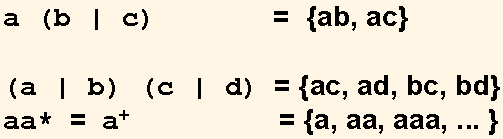
\includegraphics[width=0.38\textwidth]{c9_enzyme_re_base_01.png}}
	      \item \textcolor{red}{【重点、难点】}语法\textcolor{red}{(结合实例讲解)}
		\begin{itemize}
		  \item 选择:\verb=|=,\verb=/gray|grey/=
		  \item 数量限定:\verb|+|,\verb|?|,\verb|*|
		  \item 匹配:\verb|()|,定义操作符的范围和优先级
		\end{itemize}
	      \item \textcolor{red}{【重点】}元字符\textcolor{red}{(结合实例讲解)}
		\begin{itemize}
		  \item 简介:一个或一组代替一个或多个字符的字符
		  \item 元字符集
		  \item 元字符优先级
		    \vspace{-1em}
		    \begin{figure}[h]
		        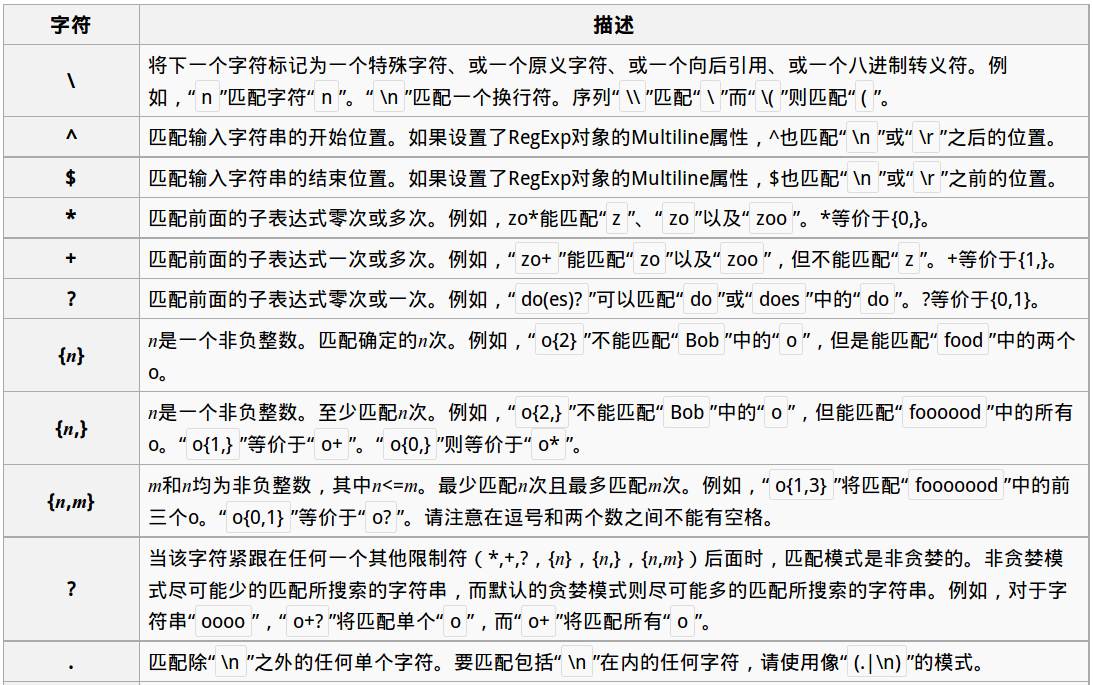
\includegraphics[width=0.6\textwidth,height=6.1cm]{c9_enzyme_re_meta_01.png}
		        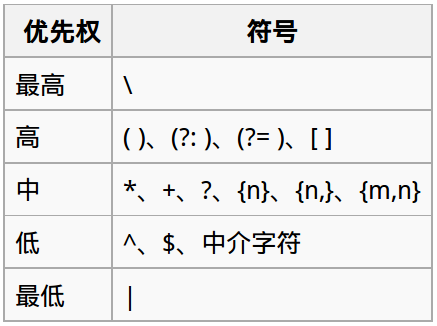
\includegraphics[width=0.4\textwidth]{c9_enzyme_re_meta_06.png}
		    \end{figure}
		    \vspace{-1em}
		\end{itemize}
	    \end{itemize}
	\end{enumerate}

\otherTail
\newpage
\otherHeader

      \item 生物学应用\textcolor{red}{(综合运用前述理论知识,讲解正则表达式在专业中的应用)}
	\vspace{-1em}
	\begin{multicols}{2}
	  \begin{itemize}
	    \item 匹配1~6号染色体
	    \item 匹配任意一个碱基/核苷酸
	    \item \textit{Bst}YI的切割序列(RGATCY)
	    \item \verb|<A-X-[ST](2)-X(0,1)-{V}|
	  \end{itemize}
	  \begin{itemize}
	    \item \verb|/chr[1-6]/|
	    \item \verb|/[ACGTU]/|
	    \item \verb|/[AG]GATC[TC]/|
	    \item \verb|/^A.[ST]{2}.?[^V]/|
	  \end{itemize}
	\end{multicols}
	\vspace{-1em}
    \end{enumerate}
  \item 限制酶切图谱(80分钟)
    \begin{enumerate}
      \item 限制酶
	\begin{itemize}
\parpic[fr]{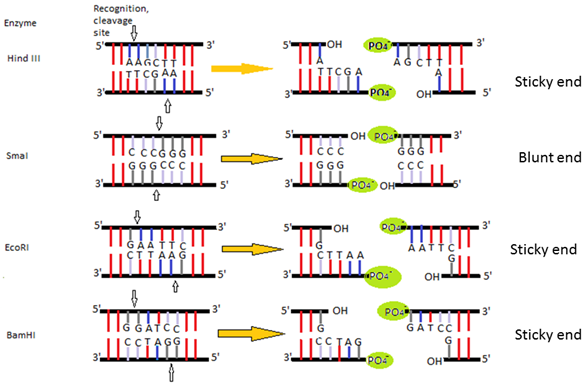
\includegraphics[width=0.5\textwidth]{c9_enzyme_eh_01.png}}
	  \item 限制酶:切割双链DNA,黏性末端或者平滑末端
	  \item 分类:Type I, Type II(回文序列), Type III
	\end{itemize}
      \item 程序规划
	\begin{itemize}
	  \item 目的:制作DNA序列酶切图谱
	  \item 输入
	    \begin{itemize}
	      \item DNA序列:读取FASTA文件
	      \item 限制酶数据:REBASE
	    \end{itemize}
	  \item 处理
	    \begin{itemize}
	      \item 表征:限制酶$\Rightarrow$正则表达式
	      \item 存储:散列(酶的名字$\Rightarrow$酶切位点)
	      \item 查询:向用户询问酶的名字
	    \end{itemize}
	  \item 输出:酶的名字,位置列表
	  \item 总结
	    \vspace{-1em}
	    \begin{multicols}{2}
	    \begin{itemize}
	      \item 限制酶翻译成正则表达式[?]
	      \item 把限制酶存储在散列中[!]
	      \item 从FASTA文件中读入DNA序列[!]
	      \item 捕获用户输入的酶的名字[!]
	      \item 根据正则表达式进行模式匹配[!]
	      \item 捕获模式匹配的位置信息[?]
	    \end{itemize}
	  \end{multicols}
	    \vspace{-1em}
	\end{itemize}
      \item 限制酶数据
	\begin{itemize}
	  \item 数据来源:REBASE数据库 $\Longrightarrow$ bionet格式的文件
	  \item 知识点:split(处理特殊变量 \verb|$_|);shift/pop(提取数组的第一个/最后一个元素)
	  \item Perl程序9.1:把IUB核酸代码转换成正则表达式
	  \item Perl程序9.2:解析REBASE中bionet格式的数据文件
	\end{itemize}
      \item 操作符
	\begin{itemize}
	    \vspace{-1em}
	    \begin{multicols}{2}
	  \item 范围操作符:\verb|..|
	  \item 逻辑操作符:and,or,not
	    \end{multicols}
	    \vspace{-1em}
	  \item \textcolor{red}{【难点】}逻辑操作符的求值顺序
	    \begin{itemize}
	      \item and:左边为真时,对右边求值返回结果;左边为假时,直接返回结果,右边永远不会被求值
	      \item or:左边为假时,对右边求值返回结果;左边为真时,直接返回结果,右边永远不会被求值
	    \end{itemize}
	\end{itemize}
      \item 制作酶切图谱
	\begin{itemize}
	  \item \textcolor{red}{【重点】}特殊变量(原字符串 = \verb|$`| + \verb|$&| + \verb|$'|)\textcolor{red}{(通过实例进行讲解)}
	    \begin{itemize}
	      \item \verb|$`|:实际匹配模式之前的部分
	      \item \verb|$&|:实际匹配模式的部分
	      \item \verb|$'|:实际匹配模式之后的部分
	    \end{itemize}
	  \item \textcolor{red}{【难点】}pos函数\textcolor{red}{(通过实例进行讲解;注意索引从0开始)}
	    \begin{itemize}
	      \item pos:返回匹配序列后面第一个字符的索引位置
	      \item pos-length:返回匹配序列第一个字符的索引位置
	    \end{itemize}
	  \item Perl程序9.3:根据用户输入的酶的名字制作酶切图谱
	\end{itemize}
    \end{enumerate}

\otherTail
\newpage
\otherHeader

  \item 操作符优先级(10分钟)
    \begin{enumerate}
      \item 优先级:操作符操作顺序的规则\textcolor{red}{(普通会员 vs. 白金会员 vs. 钻石会员)}
      \item 基本原则:使用括号明确操作顺序
    \end{enumerate}
  \item 总结与答疑(5分钟)
    \begin{enumerate}
      \item 知识点
	\begin{itemize}
	  \item 正则表达式:基础(理论、语法、元字符等);应用(解析、构建)
	  \item 操作符:范围操作符;逻辑操作符(求值顺序);优先级
	  \item 模式匹配:特殊变量,pos函数
	\end{itemize}
      \item 技能
	\begin{itemize}
	  \item 能够把IUB代码翻译成正则表达式
	  \item 能够编写制作酶切图谱相关的Perl程序
	\end{itemize}
    \end{enumerate}
\end{enumerate}

\otherTail


\end{document}
